% DO NOT COMPILE THIS FILE DIRECTLY!
% This is included by the other .tex files.

\begin{frame}{What is ELF?}
    \begin{itemize}
        \item ELF stands for Executable and Linkable Format\footnote{\url{https://refspecs.linuxfoundation.org/elf/elf.pdf}}.
        \item It is a common standard file format for executables, object code, shared libraries, and core dumps.
        \item Originally developed by Unix System Laboratories and now widely used in Unix-like operating systems.
    \end{itemize}
\end{frame}

\begin{frame}{Structure of an ELF File}
    \begin{itemize}
        \item An ELF file consists of three main parts:
        \begin{itemize}
            \item \textbf{Header:} Contains metadata about the file type, architecture, and entry point.
            \item \textbf{Program Header Table:} Describes how the file should be loaded into memory.
            \item \textbf{Section Header Table:} Provides information about the sections in the file.
        \end{itemize}
        \item ELF files are designed to be flexible and extensible.
    \end{itemize}
\end{frame}

\begin{frame}{Benefits of ELF}
    \begin{itemize}
        \item Platform-independent format, enabling portability.
        \item Simplifies the linking and loading process.
        \item Supports dynamic linking, reducing redundancy.
        \item Extensively used in modern development environments.
    \end{itemize}
\end{frame}

\begin{frame}[fragile]
\frametitle{Binwalk Output}

\begin{lstlisting}[language=bash, basicstyle=\ttfamily, breaklines=true]
Sample: 6420f5d7d48b75d687b8356e93c82721bb536c633d773f8985f74c8977425f04

binwalk sample
\end{lstlisting}

\begin{tabular}{ccp{0.6\textwidth}}
\textbf{Decimal} & \textbf{Hexadecimal} & \textbf{Description}\\
0                & 0x0                  & ELF, 32-bit LSB executable, Intel 80386, version 1 (SYSV) \\
13111            & 0x3337               & Boot section Start 0x58028941 End 0x5A41 \\
13115            & 0x333B               & Boot section Start 0x5A41 End 0x0 \\
\end{tabular}

\vspace{1cm}

$\to$ matched signatures
\end{frame}

\begin{frame}[fragile]
\frametitle{Using Binwalk}
\framesubtitle{Sample: 9e70725640c4284e2049e4b25c9cc46cca496053cebf69855ec25acc9bd63e05}
\begin{tabular}{|c|c|p{0.6\textwidth}|}
\hline
\textbf{Decimal} & \textbf{Hexadecimal} & \textbf{Description} \\ \hline
0                & 0x0                  & ELF, 64-bit LSB executable, AMD x86-64, version 1 (GNU/Linux) \\ \hline
600864           & 0x92B20              & Unix path: /usr/share/locale \\ \hline
612774           & 0x959A6              & Unix path: /usr/lib/getconf \\ \hline
620336           & 0x97730              & Unix path: /usr/lib/locale \\ \hline
622368           & 0x97F20              & Unix path: /usr/lib/locale/locale-archive \\ \hline
674903           & 0xA4C57              & Unix path: /usr/lib/x86\_64-linux-gnu/ \\ \hline

\textbf{778039}           & \textbf{0xBDF37}              & \textbf{mcrypt 2.2 encrypted data, algorithm: blowfish-448, mode: CBC, keymode: 8bit} \\ \hline
\end{tabular}

\end{frame}

\begin{frame}
\frametitle{Using Binwalk}

\begin{itemize}
    \item \textbf{Encrypted Data:}
    \begin{itemize}
        \item The file contains data encrypted using \textbf{mcrypt 2.2}.
    \end{itemize}
    \item \textbf{Encryption Algorithm:}
    \begin{itemize}
        \item Algorithm: \textbf{Blowfish-448}, a symmetric block cipher with a 448-bit key size.
    \end{itemize}
    \item \textbf{Cipher Mode:}
    \begin{itemize}
        \item Mode: \textbf{CBC (Cipher Block Chaining)} for enhanced security via block interdependency.
    \end{itemize}
    \item \textbf{Key Mode:}
    \begin{itemize}
        \item Key processed in \textbf{8-bit mode}, possibly a default for mcrypt configurations.
    \end{itemize}
    \item \textbf{Implications:}
    \begin{itemize}
        \item Decryption requires the encryption key and potentially an initialization vector (IV).
        \item Indicates sensitive or protected data within the file.
        \item Poses a reverse engineering challenge without the key.
    \end{itemize}
\end{itemize}

\end{frame}

\begin{frame}[fragile]
\frametitle{Extracting the content}
Sample: 9e70725640c4284e2049e4b25c9cc46cca496053cebf69855ec25acc9bd63e05
\begin{lstlisting}[language=bash, basicstyle=\ttfamily, frame=single, breaklines=true]
dd if=sample of=extracted_data bs=1 skip=778039
\end{lstlisting}

\begin{itemize}
    \item Binwalk uses signatures to identify and extract data from files.
    \item Determine the size of the detected block for further analysis.
    \item Evaluate whether the detection is a false positive by inspecting the data manually or using additional tools.
\end{itemize}

\end{frame}


\begin{frame}[fragile]
\frametitle{ELF Symbols from Binary Analysis}

Extract symbols from binary excluding GBLIBC references

Sample: 6420f5d7d48b75d687b8356e93c82721bb536c633d773f8985f74c8977425f04
\begin{lstlisting}[language=bash, basicstyle=\ttfamily, frame=single]
nm sample | grep -v GBLIBC
\end{lstlisting}


\begin{lstlisting}[basicstyle=\ttfamily, frame=single]
08048bfd t p4tch_sel1nux_codztegfaddczda
08048e9c t parse_cred
8050bb3 T prepare_fops_lsm_shellcode
08049215 t put_your_hands_up_hooker
0804b220 D r1ngrrrrrrr
0804988e t rey0y0code
0804b2c0 d ruujhdbgatrfe345
\end{lstlisting}
\end{frame}

\begin{frame}
\frametitle{ELF Symbols from Binary Analysis}

\begin{itemize}
    \item Interpretation of the output of tool \tt{nm}
    \item man page is your friend
\end{itemize}

\begin{tabular}{|c|p{0.7\textwidth}|}
\hline
\textbf{Symbol Type} & \textbf{Explanation} \\ \hline
a & The symbol's value is absolute and will not be changed by further linking. \\ \hline
b & The symbol is in the BSS data section. \\ \hline
d & The symbol is in the initialized data section. \\ \hline
r & The symbol is in the read-only data section. \\ \hline
t & The symbol is in the text (code) section. \\ \hline
w & The symbol is a weak symbol that has not been specifically tagged as a weak object symbol. \\ \hline
\end{tabular}

\end{frame}

\begin{frame}[fragile]
\frametitle{Using objdump to View ELF Sections}

\begin{lstlisting}[language=bash, basicstyle=\ttfamily, frame=single, breaklines=true]
objdump -h sample
\end{lstlisting}

\begin{itemize}
    \item \textbf{Output Structure:}
    \begin{itemize}
        \item Lists all sections in the ELF file, including their attributes.
        \item Provides information such as:
        \begin{itemize}
            \item \textbf{Idx}: Section index in the ELF file.
            \item \textbf{Name}: Name of the section (e.g., `.text`, `.data`).
            \item \textbf{Size}: Size of the section in bytes.
            \item \textbf{VMA (Virtual Memory Address)}: Where the section is loaded in memory.
            \item \textbf{File Off}: Offset of the section in the binary file.
            \item \textbf{Attributes}: Flags indicating section properties (e.g., `ALLOC`, `LOAD`, `READONLY`).
        \end{itemize}
    \end{itemize}
    \item \textbf{Use Case:}
    \begin{itemize}
        \item Identify key sections like `.text` (code), `.data` (initialized data), `.bss` (uninitialized data), and `.dtor` (destructors).
        \item Useful to identify the type of binary, such as a C program, C++, Go (Golang), etc. 
    \end{itemize}
\end{itemize}

\end{frame}



\begin{frame}[fragile]
\frametitle{ELF Section Details}

\begin{tabular}{clcccp{1cm}}
\textbf{Idx} & \textbf{Name}       & \textbf{Size}  & \textbf{VMA}     & \textbf{LMA}     & \textbf{File Off} \\
0            & .interp            & 00000013       & 08048134         & 08048134         & 00000134          \\
1            & .note.ABI-tag      & 00000020       & 08048148         & 08048148         & 00000148          \\
2            & .gnu.hash          & 00000030       & 08048168         & 08048168         & 00000168          \\
3            & .dynsym            & 00000290       & 08048198         & 08048198         & 00000198          \\
11           & .text              & 00001788       & 080489b0         & 080489b0         & 000009b0          \\

\end{tabular}

\vspace{1cm}

\begin{tabular}{cc}
\textbf{Idx} &  \textbf{Attributes}\\
0            &  CONTENTS, ALLOC, LOAD, READONLY, DATA \\
1            &  CONTENTS, ALLOC, LOAD, READONLY, DATA \\
2            &  CONTENTS, ALLOC, LOAD, READONLY, DATA \\
3            &  CONTENTS, ALLOC, LOAD, READONLY, DATA \\
11           &  CONTENTS, ALLOC, LOAD, READONLY, \textbf{CODE}
\end{tabular}

\end{frame}


\begin{frame}
\frametitle{Collaborative Malware Analysis Using MISP}

\centering
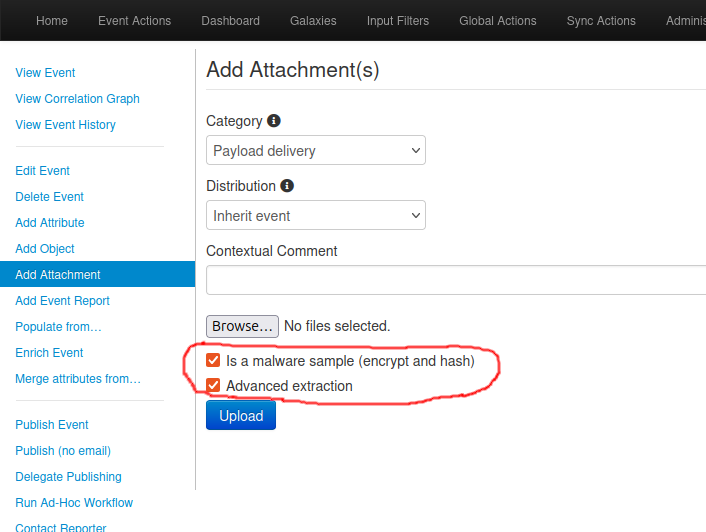
\includegraphics[width=0.8\textwidth]{img/upload2.png}

Uploading your sample to MISP

\end{frame}

\begin{frame}
\frametitle{Collaborative Malware Analysis Using MISP}

\centering
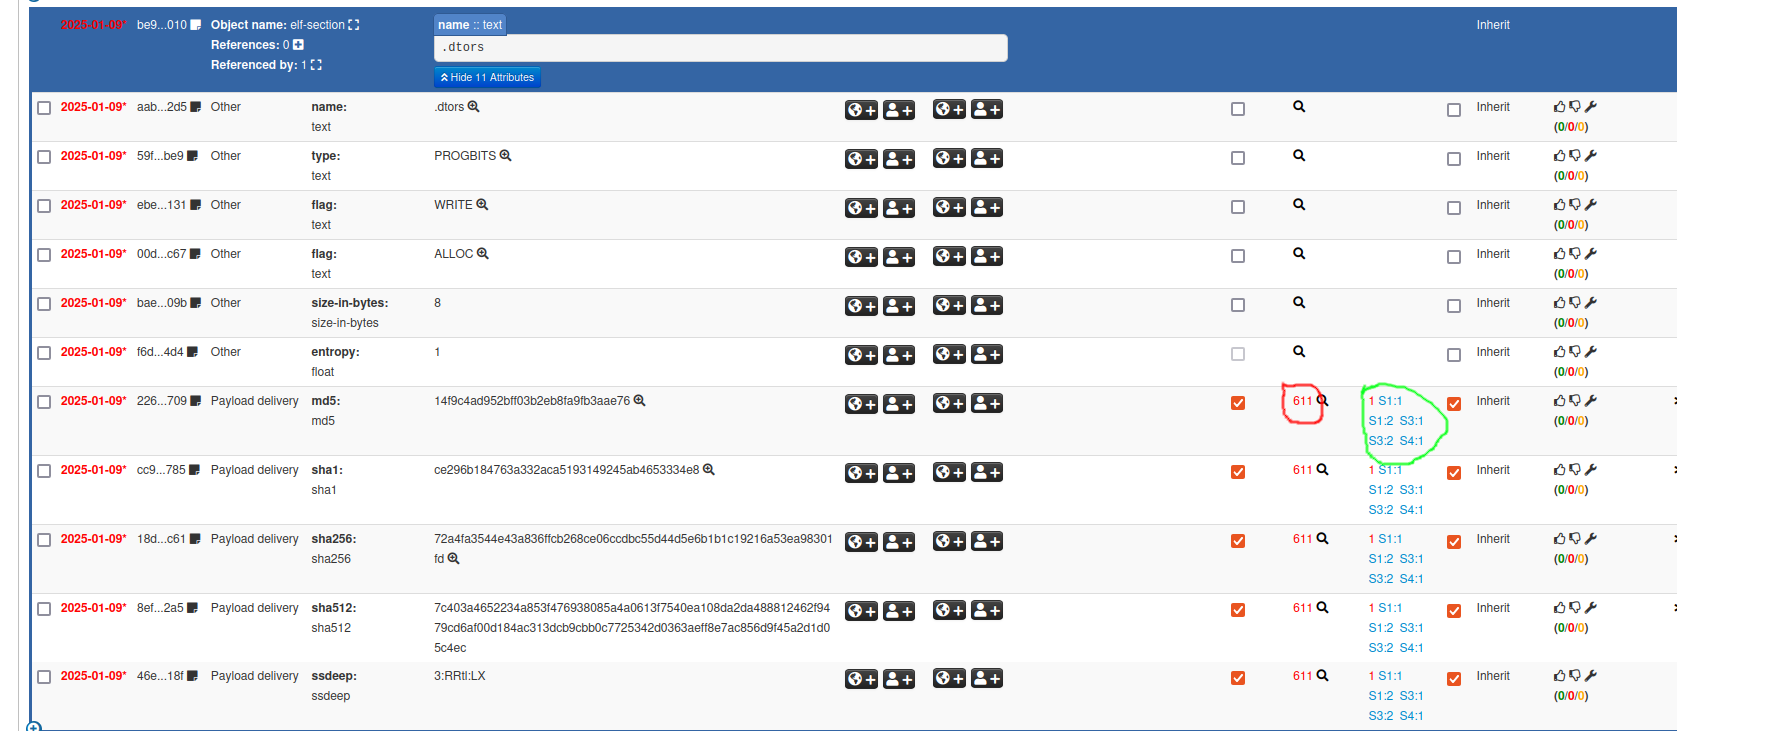
\includegraphics[width=0.8\textwidth]{img/correlation2.png}

\begin{itemize}
    \item Explore correlations between events and indicators.
    \item Analyze hits from threat intelligence feeds.
    \item Review hits from synchronization caches.
\end{itemize}

\end{frame}

\begin{frame}
\frametitle{Collaborative Malware Analysis Using MISP}

Exploring connected MISP instances within MISP-LEA

\centering
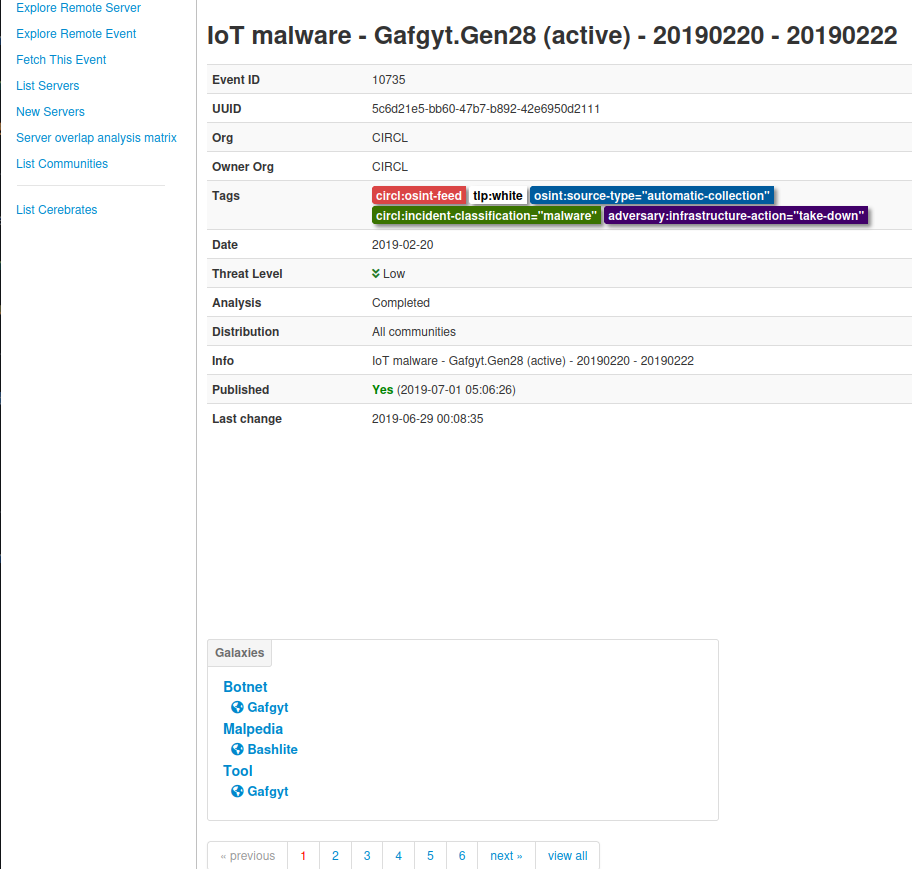
\includegraphics[width=0.6\textwidth]{img/foreign.png}

\end{frame}

\begin{frame}
\frametitle{Introduction Ghidra}

\begin{itemize}
    \item \textbf{Disassembly and Decompilation:}
    \begin{itemize}
        \item Transforms binary code into human-readable assembly.
        \item Generates high-level language representations (C-like pseudocode).
    \end{itemize}
    \item \textbf{Cross-Platform Support:}
    \begin{itemize}
        \item Analyzes binaries for multiple architectures (x86, ARM, MIPS, etc.).
        \item Compatible with various operating systems (Windows, Linux, macOS).
    \end{itemize}
    \item \textbf{Collaboration:}
    \begin{itemize}
        \item Supports multi-user reverse engineering projects.
        \item Version-controlled changes for shared analysis.
    \end{itemize}
    \item \textbf{Scriptability:}
    \begin{itemize}
        \item Customize and automate analysis with Python and Java.
    \end{itemize}
    \item \textbf{Extensibility:}
    \begin{itemize}
        \item Add plugins and extend functionality for specific needs.
    \end{itemize}
    \item \textbf{Data Flow Analysis:}
    \begin{itemize}
        \item Tracks variables, functions, and references for better insight.
    \end{itemize}
\end{itemize}

\end{frame}

\begin{frame}
\frametitle{Static Analysis Using Ghidra}
\begin{itemize}
    \item Creating a project in Ghidra.
    \item Importing and analyzing a binary file.
\end{itemize}

\centering
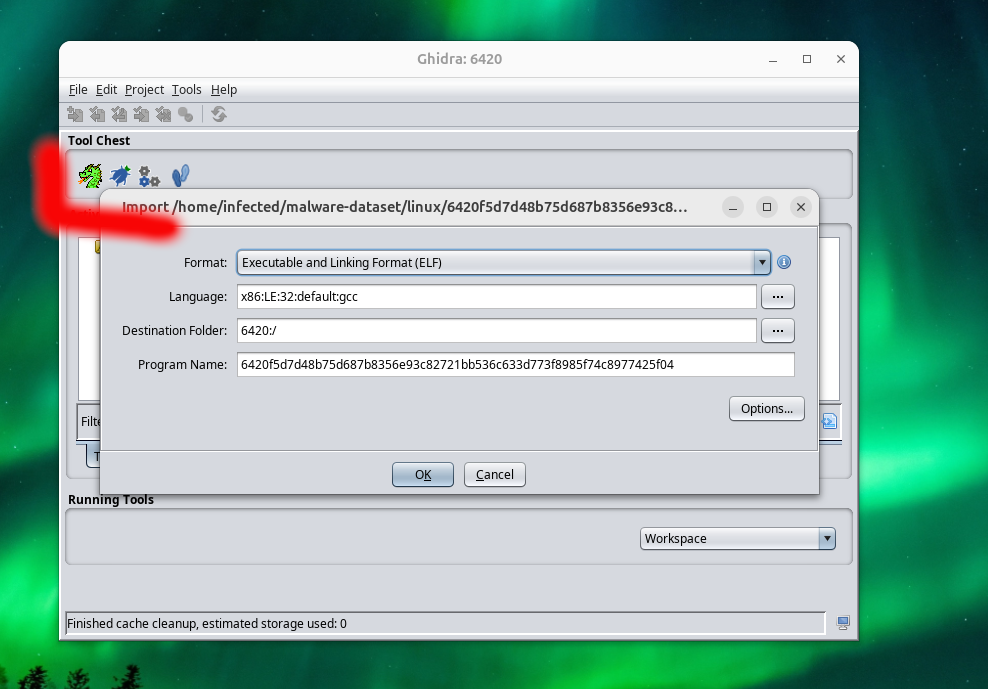
\includegraphics[width=0.6\textwidth]{img/g0.png}

\end{frame}

\begin{frame}
\frametitle{Static Analysis Using Ghidra}

\begin{itemize}
    \item Determine the type of binary (e.g., ELF, PE).
    \item Analyze the binary's metadata for key attributes such as architecture, endianness, and sections.
\end{itemize}

\centering
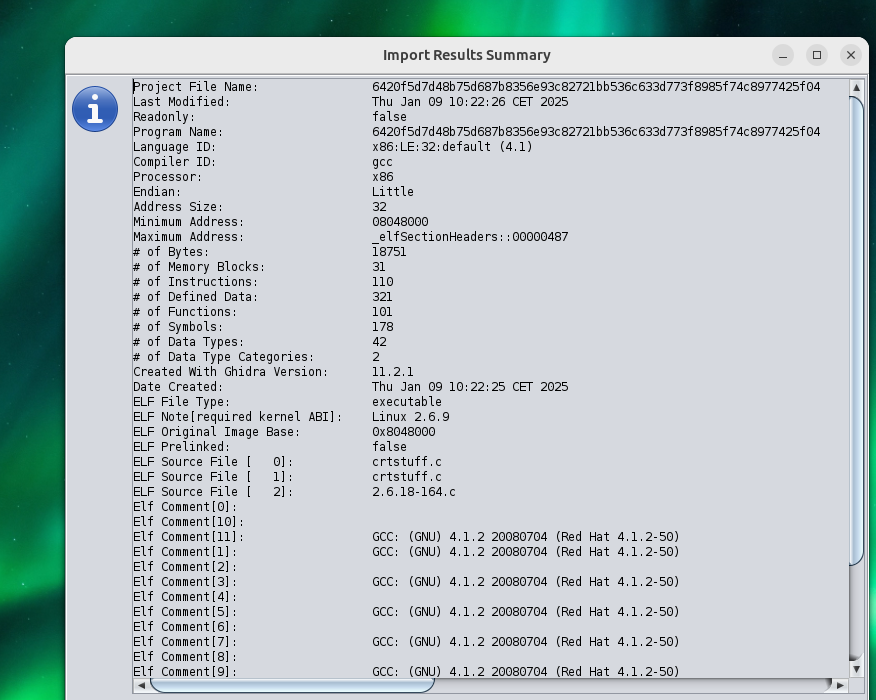
\includegraphics[width=0.6\textwidth]{img/g1.png}
\end{frame}

\begin{frame}
\frametitle{Static Analysis Using Ghidra}

\begin{itemize}
    \item Explore the functions defined within the binary.
    \item Analyze the disassembly view to examine low-level instructions.
    \item Utilize the decompiled view for a high-level representation of the code.
\end{itemize}

\centering
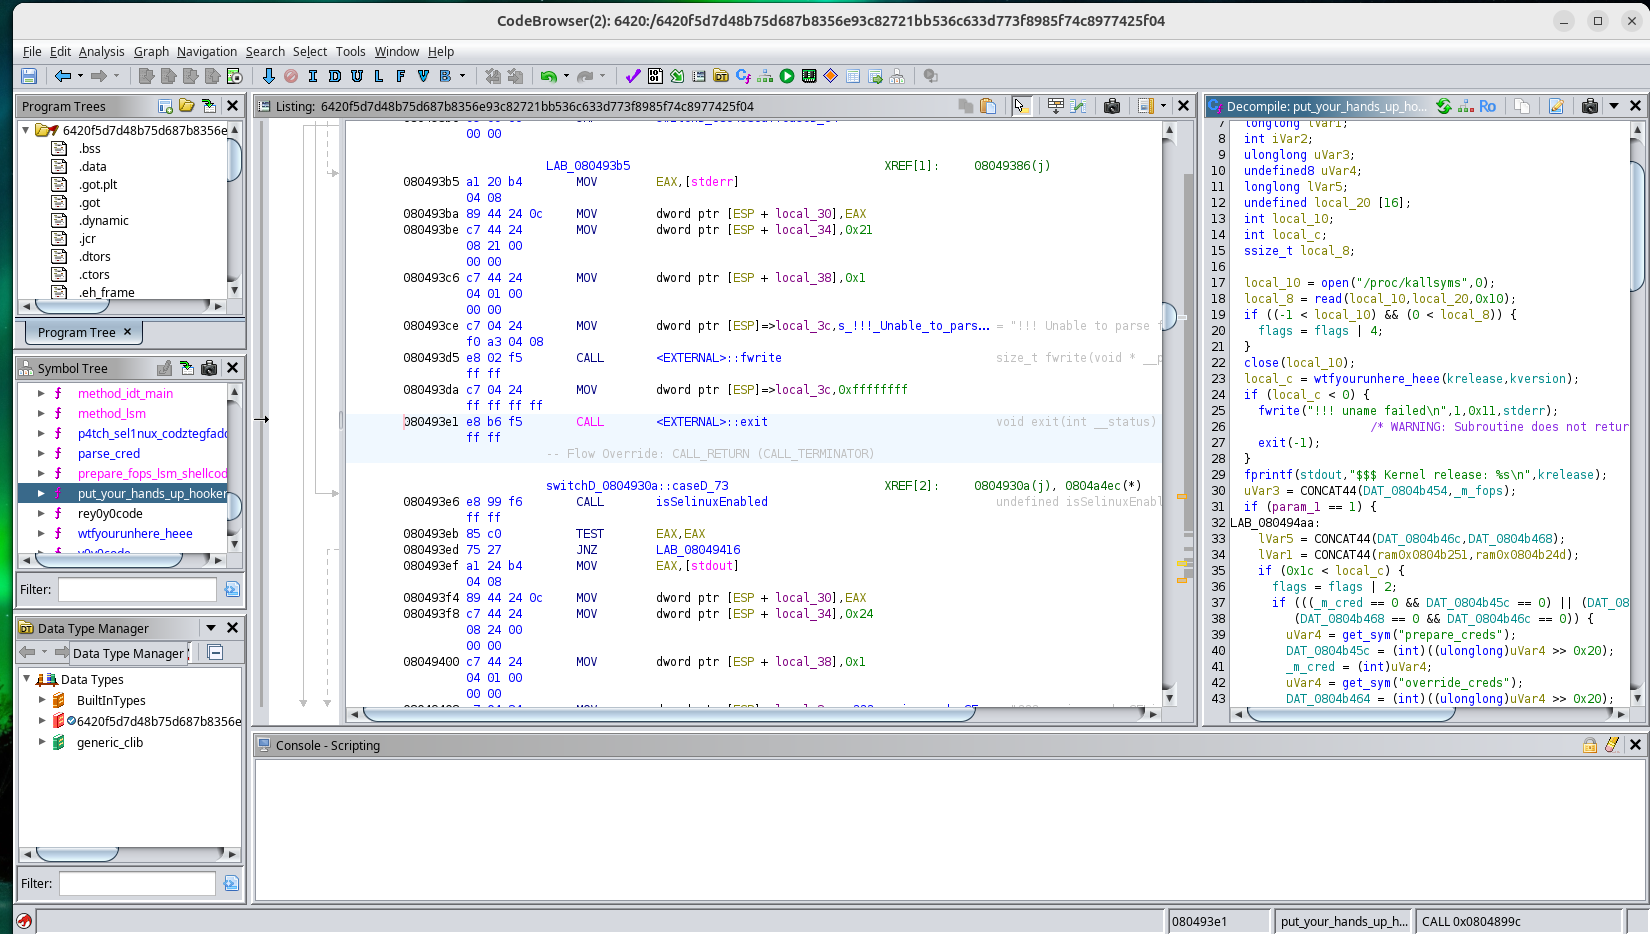
\includegraphics[width=0.6\textwidth]{img/g2.png}
\end{frame}

\begin{frame}
\frametitle{Static Analysis Using Ghidra}

\begin{itemize}
    \item \textbf{Benefits of Ghidra's Decompiled View:}
    \begin{itemize}
        \item Provides a high-level, human-readable representation of the code.
        \item Simplifies understanding of complex binaries.
    \end{itemize}
    \item \textbf{Avoid Manual Pattern Matching:}
    \begin{itemize}
        \item Eliminates the need to manually match patterns in assembly code.
        \item Speeds up the reverse engineering process.
    \end{itemize}
\end{itemize}

\centering
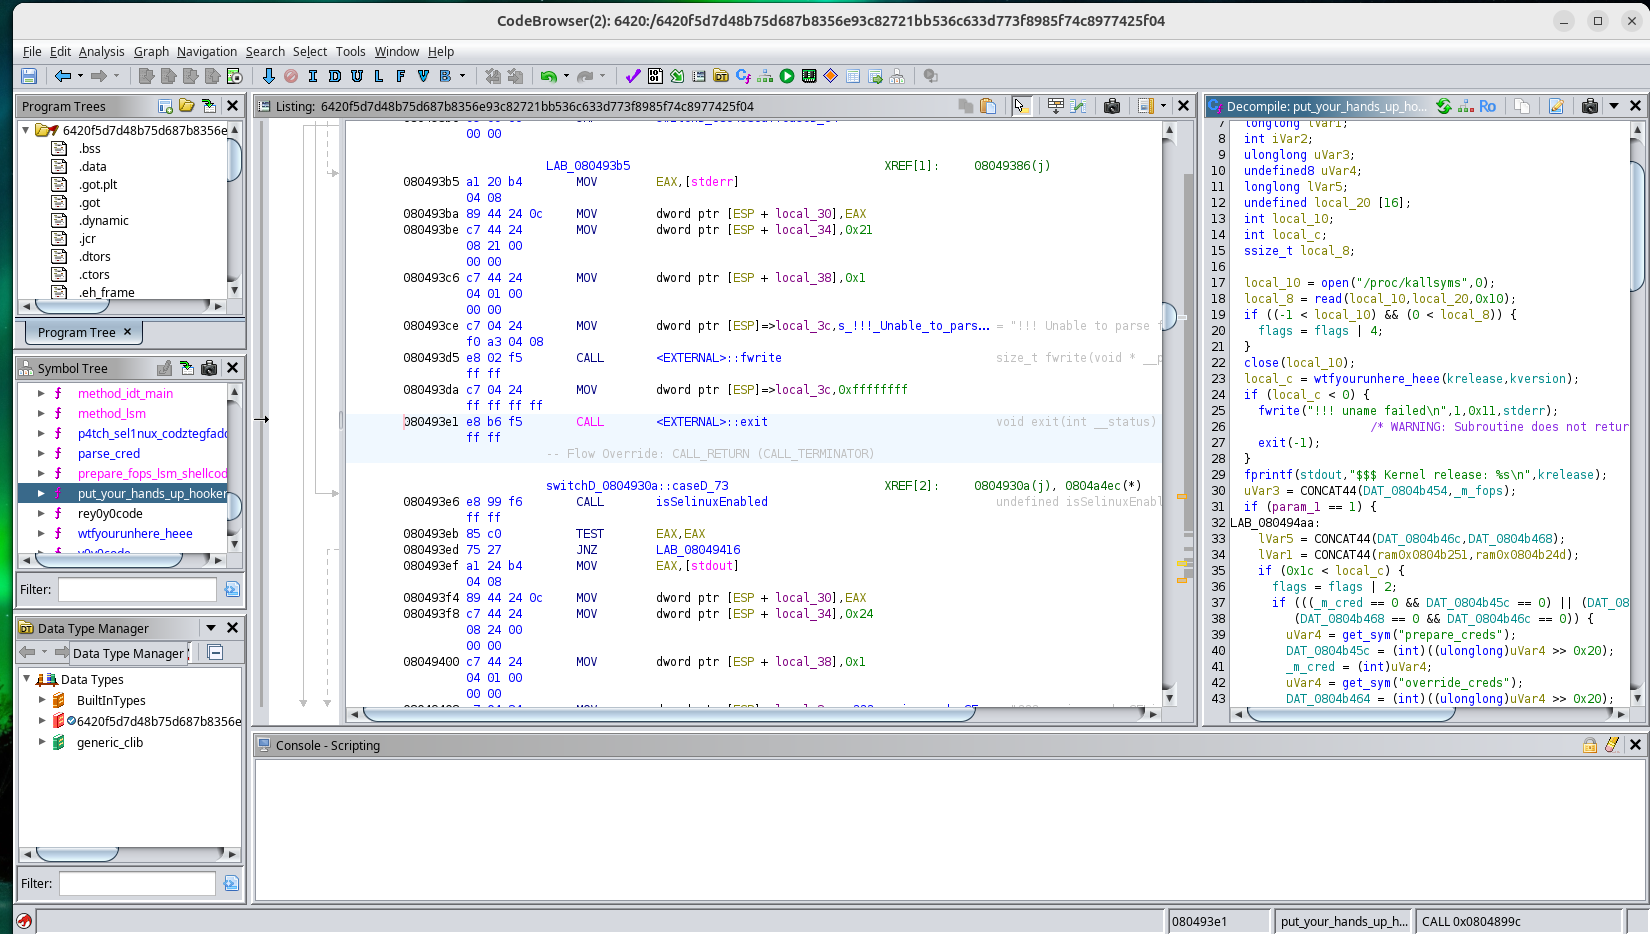
\includegraphics[width=0.6\textwidth]{img/g2.png}
\end{frame}

\begin{frame}
\frametitle{String Analysis and Cross-References in Ghidra}

\begin{itemize}
    \item Identify interesting strings, such as filenames, hardcoded paths, or error messages.
    \item Use the cross-references (Xrefs) feature to determine which functions or code sections utilize these strings.
\end{itemize}

\centering
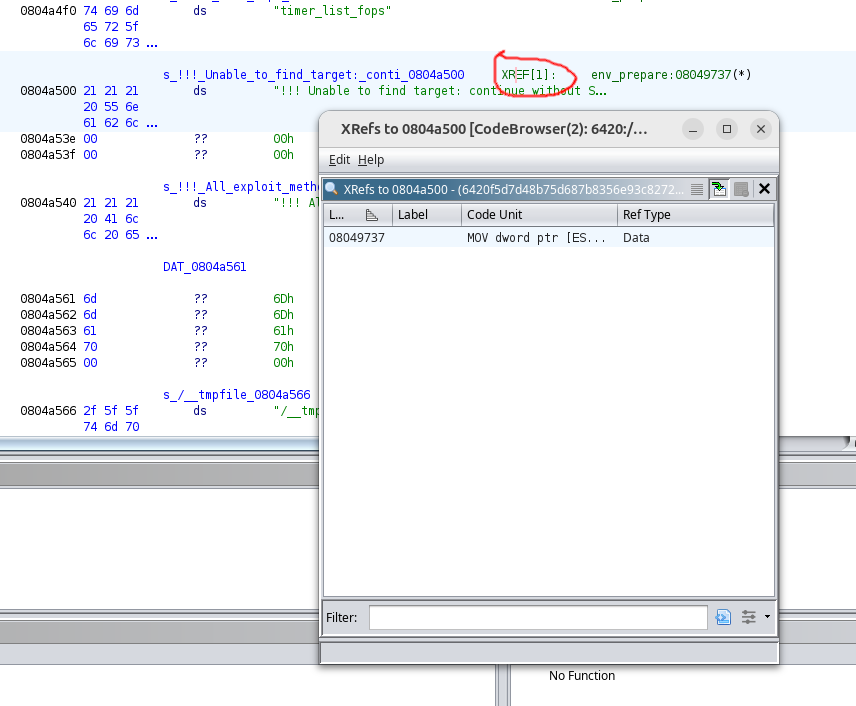
\includegraphics[width=0.6\textwidth]{img/gxref.png}
\end{frame}
